\documentclass[convert={density=300,size=1080x800,outext=.png}]{standalone}

\usepackage[latin1]{inputenc}
\usepackage{tikz}
\usetikzlibrary{shapes,arrows}
\usetikzlibrary{calc}

\begin{document}


\centering
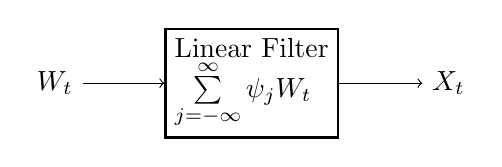
\begin{tikzpicture}[node distance=2.5cm, auto]
\node (error) {$W_t$};
\node[rectangle, right of=error, align=left] (filter) [fill=none, draw = black, thick] {Linear Filter \\ $\sum\limits_{j = -\infty}^{\infty}{\psi_jW_t}$};
\node[right of=filter] (obs) {$X_t$};

\draw[->]
  (error) edge (filter) (filter) edge (obs);
\end{tikzpicture}

\end{document}